\section{Product perspective}
The basic idea upon which the system will be built is that the user is a
volounteer, so it has to put as little effort as possible to send information
about violations.

Right after the user enters the application, he can take a picture directly from
there. Then the taken picture is scanned by an OCR algorithm that detects (or at
least tries to) the biggest licence plate and obtains its number. The
application proceeds to collect as much data as possible from the built-in
functions of the host device: gets the time, date and retrieves location through
GPS.
The auto-collected data is then showed to the user who can correct or
complete it. Finally the user inserts the infraction type and the violation is
ready to be sent to the authorities.
When sending the violation to the authority the system doesn't save the name
of the user on the violation itself, in order for it to remain anonymous.

In figure \ref{fig:classDiagram} we represent the main entities of interest
for the system.
A \emph{Violation} is reported by exactly one \emph{User}. It is associated to
exactly one \emph{Picture}, \emph{Location} and \emph{Vehicle} that commited it;
these have no reason to be considered by the system if they are not associated
to at least one violation.

\emph{Accidents} are also associated to their \emph{Location}, so the system can
match them with \emph{Violations} to provide \emph{SuggestedActions} in order
order to reduce accidents.

A \emph{Location} where a violation or accident took place belongs to exactly
one municipality. In the real world, each municipality has an authority which is
responsible for it, however we used the $0..1$ cardinality to represent the
fact that the authority might not participate to SafeStreets; in this case, it
makes no sense for users to report violations in that area.

Each authority might have multiple operators which are allowed to handle the
violations reported in its competence area.

% Insert class diagram
\begin{figure}[H]
    \centering
    \includegraphics[width=0.75\linewidth]{rasd_class_diagram}
    \caption{Class diagram}
    \label{fig:classDiagram}
\end{figure}

Figure \ref{fig:violationDiagram} shows the evolution of a Violation, from when the user takes the picture, to the final user review.

% Insert state_diagram_violation
\begin{figure}[H]
    \centering
    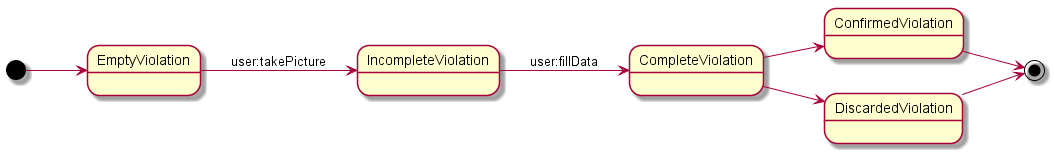
\includegraphics[width=\linewidth]{../diagrams/state_diagram_violation.png}
    \caption{Violation state diagram}
    \label{fig:violationDiagram}
\end{figure}

Notice that depending on the quality of the picture taken, the OCR algorithm may fail, in this case the user is asked to take another, possibly better, picture. 

Figure \ref{fig:acceptViolationDiagram} shows what happens when an operator takes care of a Violation that is received by the authority. As explained before, firstly it has to accept or discard the violation, then in case of acceptance assign it a level of priority so that another department can better schedule the intervention

% Insert state_diagram_accept_violation
\begin{figure}[H]
    \centering
    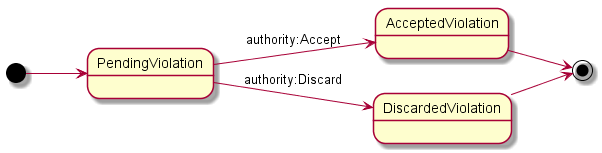
\includegraphics[width=\linewidth]{../diagrams/state_diagram_accept_violation.png}
    \caption{Accept Violation state diagram}
    \label{fig:acceptViolationDiagram}
\end{figure}